
\msection{Attentional Filtering (Objective 3) }
\label{sec:aim3}

More information is available to our senses than the brain can
handle. As a result, we process only a subset of this information and
this determines what enters conscious
awareness~\citep{Most:2005}, what we learn
~\citep{Turk-Browne:2005}, and what we store in
memory~\citep{Aly:2016}. The mechanisms governing the
selection of sensory information are referred to as the study of
\textit{attention}. An analogous problem, known as the curse of
dimensionality, arises in statistical machine learning for
high-dimensional problems. As with human attention, reducing the
dimensionality of data can make learning tractable. Here we will
explore whether our understanding of attention in cognitive
neuroscience can inform assumptions made in machine learning, and how
techniques for recovering lower-dimensional representations in machine
learning can be used to reconstruct fluctuations in human attention
from brain imaging data.

\biobackground{} Attention in the human brain can be controlled
reflexively by the salience of stimuli, including their 
contrast or motion~\citep{Itti:2000}. This
stimulus-driven, bottom-up form of attention explains how our focus
is automatically drawn to an approaching siren or to a screen
lighting up with a text message. It can be distinguished from
goal-directed, top-down attention, whereby we volitionally shift 
focus based on which stimuli are relevant for current behavioral
goals~\citep{Yantis:2000}. In both stimulus-driven and goal-directed
forms, attention is directed at external stimuli, enhancing evoked
activity in brain areas that code for their locations and
features~\citep{Kastner:2000} and increasing functional connectivity
between these areas~\citep{Turk-Browne:2013}. This modulation occurs
as a result of control structures in frontoparietal cortex that send
biasing signals to visual cortex~\citep{Noudoost:2010}. Attention can 
also be directed toward internal representations, such as
thoughts or memories, and this is mediated by similar
neural control mechanisms~\citep{Chun:2011}. This internal
attention, as well as goal-directed external attention, share the
fascinating property that are not determined by the appearance of the
world. Rather, they reflect computations in the mind and allow each
individual to process the same sensory input in different ways. The
challenge for understanding these forms of attentional filtering is
being able to characterize the inner mental life of a person, even in
cases where they do not (or cannot) disclose their focus.

Methods have been developed in recent years to infer
mental experience from brain data, including
colors~\citep{Brouwer:2009}, scenes~\citep{Naselaris:2009},
faces~\citep{Cowen:2014}, and locations~\citep{Sprague:2016}. The
steps involved in such reconstruction or inverted encoding models
involves: (1) specifying a basis set of channels that tile the
dimension to be reconstructed; (2) predicting the activation of each
channel given the position of each stimulus used in the experiment on
that dimension; (3) for a training set of fMRI data, modeling the
observed neural responses to these stimuli in each voxel as a weighted
sum of the predicted channel activations; (4) this results in an
estimated weight matrix of the extent to which each channel is encoded
in each voxel, from which a tuning curve for each voxel can be
computed as a weighted sum of the basis set; (5) by inverting this
estimated weight matrix, test fMRI data with the pattern of neural
responses across voxels for an unknown stimulus can be used to
estimate channel activation; (6) the weighted sum of these estimated
channel activations by the basis set provides a continuous readout of
the information present in the brain along the dimension of interest,
which can be used as is or for decoding by finding the stimulus whose
predicted channel activations (from step 2) are most correlated.

\setlength{\columnsep}{20pt}
\begin{wrapfigure}{R}{0.48\textwidth}
\centering
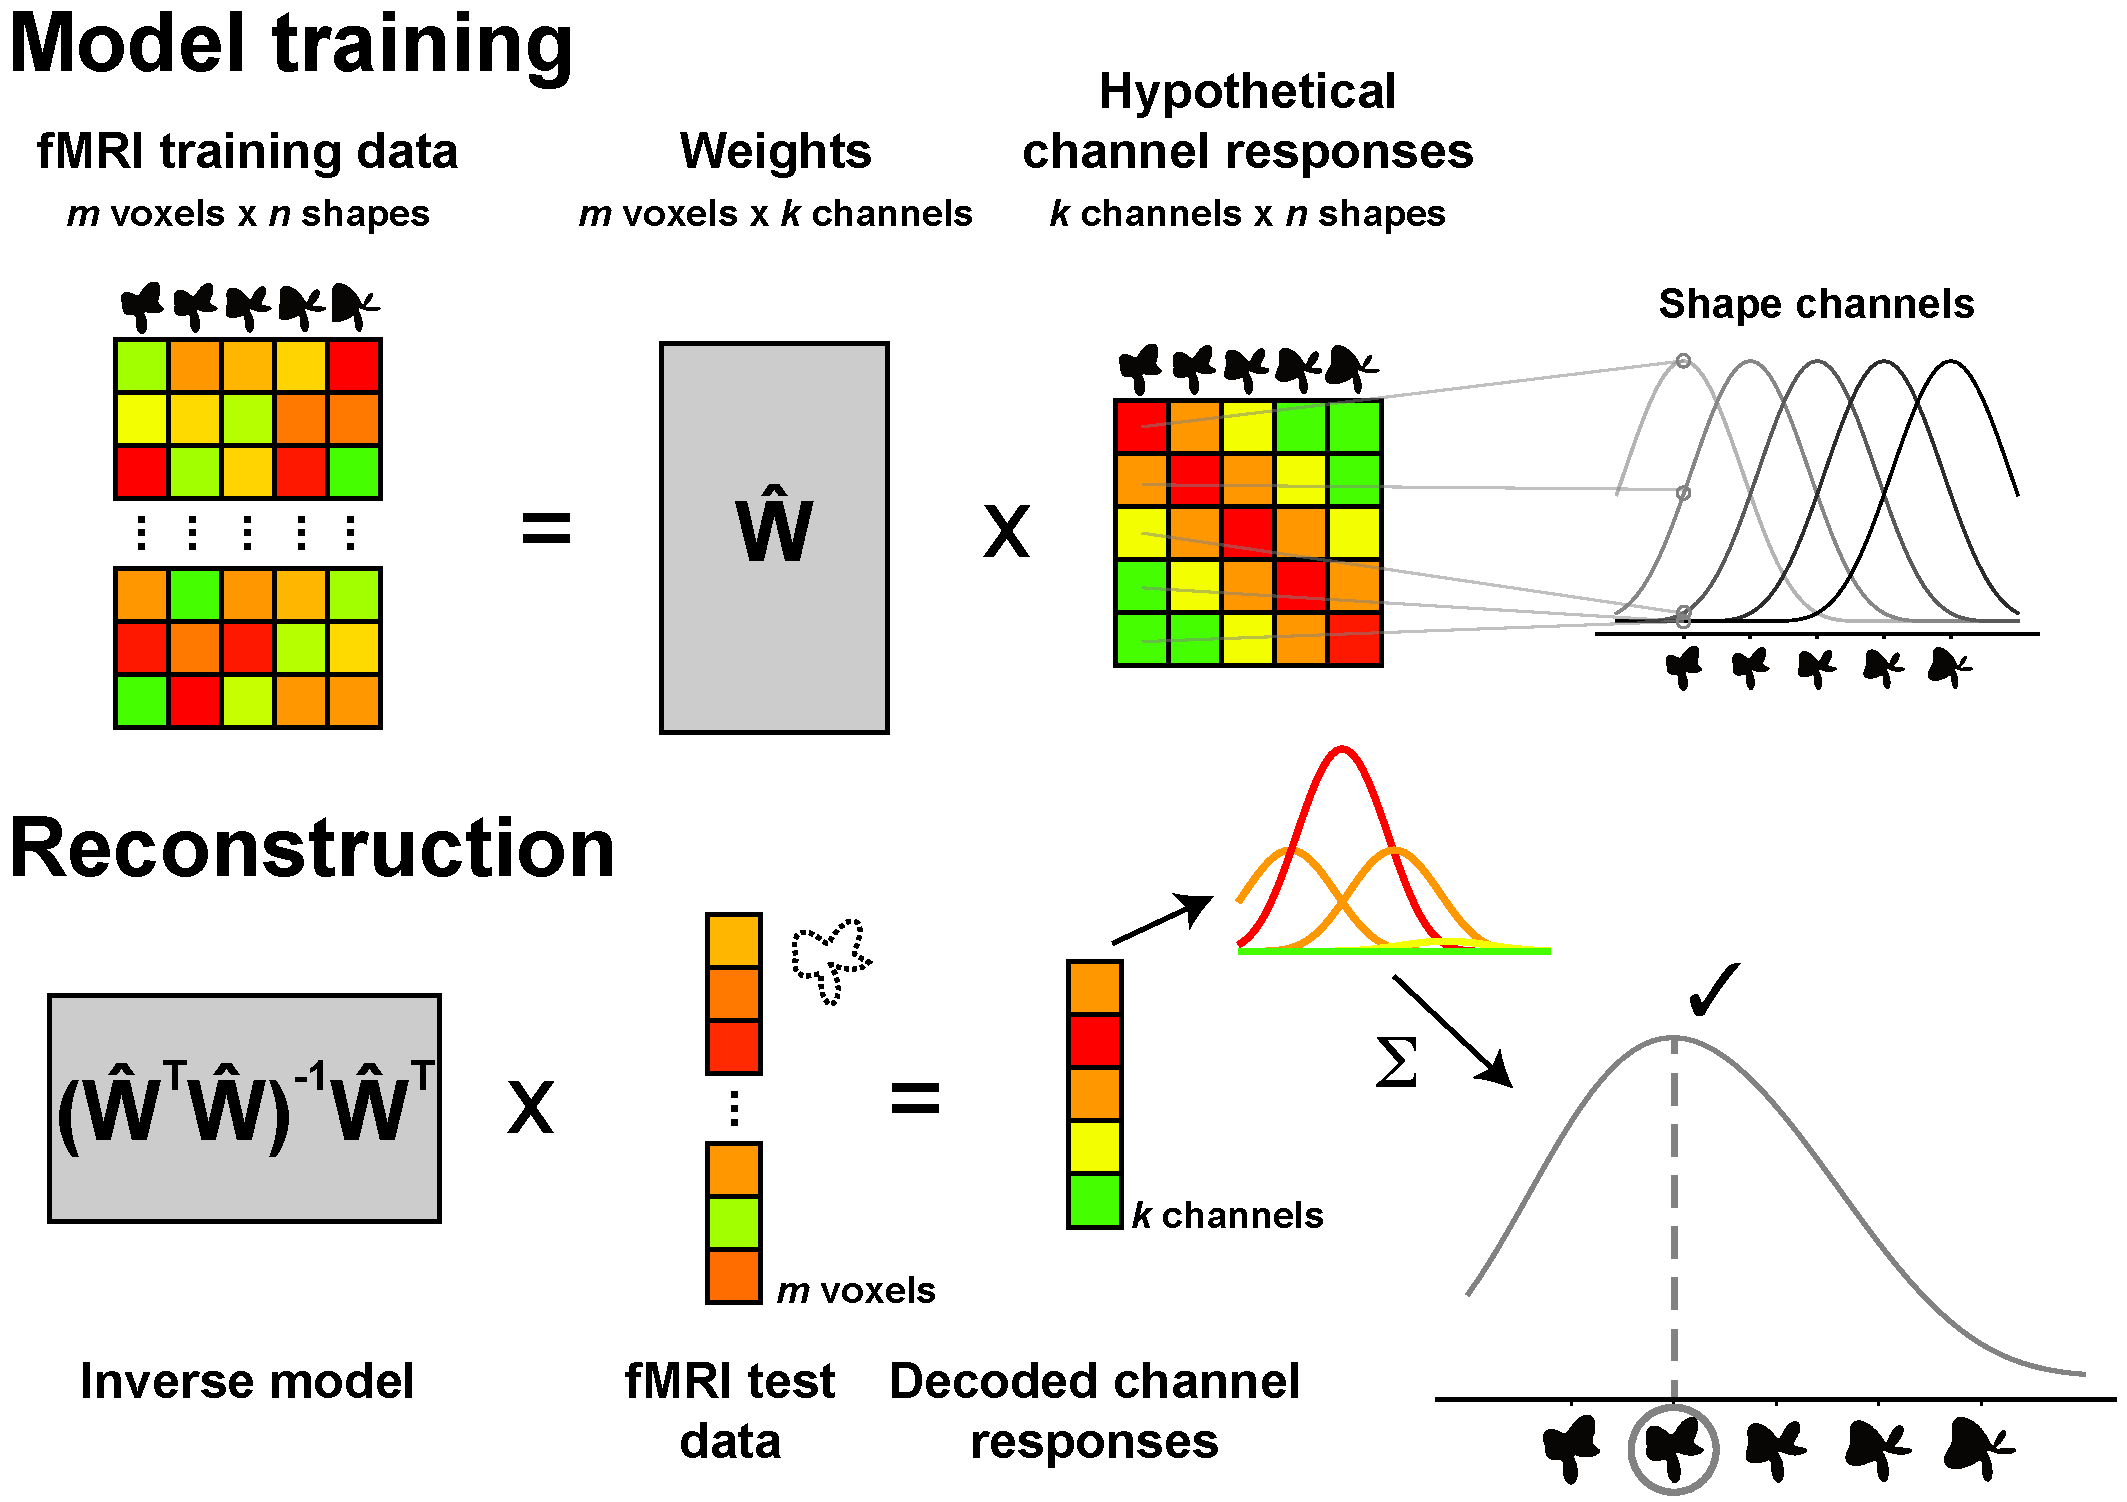
\includegraphics[width=.48\textwidth]{figs/inverse}
\caption{\small Example reconstruction analysis. Linear regression was
used to learn the tuning of voxels over a continuous space of novel
Fourier descriptor shapes. The inverse of the resulting weight matrix
was used to estimate the shape information present in a pattern of
activity over voxels in a brain region during a separate task in which
human subjects predicted which shape would appear on each trial.
In this study, shapes could be reconstructed from visual cortex and
hippocampus~\citep{Kok:2018}.}
    \label{fig:hippo}
    \vskip2pt
\end{wrapfigure}

Although these methods are cutting-edge and powerful in cognitive
neuroscience, and they come tantalizingly close to ''mind reading'',
they are currently limited in two ways. First, they require an
assumption (for training and decoding) that the brain veridically
represents the properties of the stimulus used as labels (e.g., known
visual or semantic features). To the extent that attention filters the
stimulus in some way, this changes the ground truth about which
features the brain should be representing, inherently limiting
reconstruction accuracy. Second, these methods are generally applied
to stimuli with one or a small number of potential dimensions that are
used for reconstruction. However, naturalistic stimuli are
high-dimensional and dynamic, increasing the likelihood that people
are shifting their attention between dimensions. We will thus extend
these approaches by attempting to reconstruct from brain activity not
only what stimulus information is present in each dimension but also
to which dimension(s) attention is directed. We will deploy methods
from machine learning that can uncover lower-dimensional traces
through high-dimensional data to infer how attention is filtering the
stimulus, even when the attentional focus during the training data is
unknown (i.e., it was not manipulated or measured). Our
overall goal is to improve decoding accuracy by reconstructing what is
represented in the mind rather than what is presented to the eyes.


\statbackground{} High-dimensional problems suffer from the curse of
dimensionality. This has a precise mathematical characterization in
standard models of statistical machine learning. The curse of
dimensionality has two components, one statistical, the other
computational. The statistical issue stems from the observation that
in high dimensions, any local ball will contain very few data
points. The computational curse is implied by the fact that searching
over a sufficiently large space of models is often
intractable. ``Beating'' the curse of dimensionality involves making
assumptions about the structure of the learning problem, and then
developing estimation and inference algorithms that provably 
recover that structure, with fast running times. The most prominent 
example in statistics in recent years is the assumption of sparsity, and the explosion of methods based on regularization that recover sparse signals \citep{Tibs:1996,lars,Wain:09a,wasserman:09,Zou:Hastie:Tibs:05,FHT:07}; methodology has also been developed for nonparametric problems \citep{LZ:Cosso,Ravikumar:08,lafferty2008rodeo,NPN:09,skeptic,NRRR:NIPS}

We will study mathematical formulations of attention as one approach
to making assumptions for which learning is tractable in principle.
In an attention-based model, the object of study is a
lower-dimensional trace or curve through the high-dimensional input
space. While the family of curves may be infinite dimensional, a
locally sparse or ``focused'' representation is intended to make
learning statistically and computationally tractable. Rudimentary
versions of this notion appear in the machine learning literature in
different forms.  For example, sparse coding representations have
been extended to be based on hierarchical and local coding schemes
\citep{WangYYLHG10,YuLL11}, and hierarchy and context have been 
incorporated into image models \citep{ChangJZBG11,JinG06}. In the
deep learning literature, attention-based models were first developed
in the setting of machine translation, using sequence-to-sequence
algorithms based on recurrent neural networks
(RNNs) \citep{bahdanau2014}. The attention mechanism is a type of
alignment model, which is a key component of statistical translation
methods \citep{Brown1993}. Attention has been applied to the problem of generating image
descriptions by \cite{showtell}.

\project{Attention-based latent embedding models}
We will investigate the introduction of the attention-based metaphor into
statistical learning using exponential family embedding models, latent
variables, and multiple embedding characteristics as described in
Objective 2 above. 
Recall from above that an exponential family embedding model uses a
latent representation of the input and output variables. Consider the
case of high dimensional density estimation, where the goal is to
estimate a density $p(x)$ for $x\in\reals^d$.  A latent variable
embedding model takes the form
$$ p(x) = \int p(z) \exp(\rho(x)^T \alpha(z) - \Psi_{\rho,\alpha}) \, dz$$
where $z\in \reals^m$ is a latent Gaussian vector,
$\rho:\reals^d \to \reals^K$ is an embedding of the input space,
and $\alpha: \reals^m \to\reals^K$ is an embedding of the latent
Gaussian, and $\Psi_{\rho,\alpha}$ is a normalizing constant.
In an attention-based model, we would consider a parameterized curve $t\mapsto (Z_t, S_t)$
where $Z_t$ is a Gaussian vector and $S_t \subset \{1,\ldots, d\}$
is a subset of the input variables. Define the inner product 
$\langle x, z\rangle_{\rho,\alpha}
= \int_{0}^1 \rho\left(x_{S(t)}\right)^T \alpha(Z_t) dt,$
and the corresponding embedding model
$ p(x) = \int \exp\left(\langle x, z\rangle_{\rho,\alpha} - \Psi_{\rho,\alpha}\right) d\mu(z)$ where $\mu(z)$ is a 
measure over ``attention paths,'' for example defined in terms of a Gaussian process.
In another version, consider a graph over $\{1,\ldots, d\}$ with edge
set $E$, and define the inner product
$\langle x, z\rangle_{\rho,\alpha}
= \sum_{(j,k)\in E} \rho(x_j, x_k)^T \alpha(Z_j, Z_k)$
where $Z$ is now a vector-valued Gaussian random field, 
and the model can be viewed as a nonparametric graphical model
\citep{hl18}. Returning to the discussion of data representation (Objective 2), 
if $Z(t)$ is an embedding having different components corresponding
to appearance, function, reward, and co-occurrence, then $S(t)$ might 
indicate attending to those different latent dimensions in turn.

These are thought of as attention-based models as the ``energy''
$\langle x, z\rangle_{\rho,\alpha}$ is localized to subsets of the
sample space or components of the latent variables. Discriminative or regression-based versions of these
models are defined similarly. The project will develop variational
inference algorithms for this family of models. When the mapping 
$\alpha(z)$ is defined in terms of, for instance, a feed-forward
neural network, this can be viewed in the framework of variational auto-encoders
\citep{kingma13}.


\project{Applications to fMRI movie data}
The public movie dataset mentioned earlier consists of 17 subjects
watching a 90-minute episode of BBC's Sherlock while being scanned with
fMRI~\citep{chen17,baldassano17}. We also have a frame-by-frame
annotation of several dimensions of the movie, including: scene
location, characters present, speaker, camera angle, music, arousal, and
valence (i.e., positive or negative mood). Consider the task of
reconstructing a person's subjective experience of the movie from their
brain data. As described above, existing inverse modeling methods
attempt to reproduce the visual or auditory stimulus presented to the
subject. However, for naturalistic stimuli like a movie with multiple
dimensions present, the limited capacity of human attention to a small
number of dimensions ensures that this reproduction will fail. We are
likely to only experience a subset of the input and which subset we
experience will change over time. There are currently no principled
techniques for characterizing this internal ''ground truth''. We will
exploit this annotated dataset to align the different dimensions of the
movie with the fMRI time series. Using an attention-based and dynamic
exponential family embedding model with multiple embeddings, we will
attempt to read out the attentional trace of the observer over time.


\project{Learning complexity under attention}
Classical statistical theory characterizes the complexity of
estimation and inference tasks in terms of minimax rates of
convergence. Parametric problems have risk (expected squared error)
that scales as $R_n \asymp p/n$ when there are $p$ parameters and $n$
samples. In the high dimensional sparse regime, research over the past
decade has shown that the risk scales as $R_n \asymp s \log p/n$ 
in a rich array of settings, where $s$ is the intrinsic dimension or
sparsity level. For nonparametric sparse additive
models \citep{Ravikumar:08}, it is known that the risk
scales (informally) as $\tilde O(s n^{-\alpha})$ where $n^{-\alpha}$ is 
the minimax rate for the underlying function space;
e.g., for an $m$-th order Sobolev space we have
$\alpha = 2m/(2m+1)$. These complexity results can be established using
the tools of empirical process theory, covering numbers, and metric
entropies. We will consider a series of mathematical formalizations
of attention, and investigate corresponding minimax rates of 
convergence, and bounds on approxmation errors in different settings.
As a concrete example, consider a regression model where the regression function 
has an attention component, expressed as 
$$ \E(Y\given x) = \int f(A_t^T x_{S_t}) \, dt.$$
This can be considered as a form of semiparametric single-index model
\citep{horowitz09,horowitz96,ichimura93,kakade11,negahban12} 
and we anticipate that we can characterize
the minimax complexity of estimating such models. We will also investigate
the theory of latent variable attention models.





 
